\RequirePackage[T1]{fontenc}
\documentclass[conference,10pt]{IEEEtran}
\usepackage{amsmath,amssymb,graphicx,url}
\title{Current-STA Transactional Repair for Timing--Resource Tradeoffs in 3D FPGA Routing}
\author{\IEEEauthorblockN{Anonymous development manuscript}}
\begin{document}
\maketitle
\begin{abstract}
Legal routing trades timing, wire and vertical resources. Current-STA transactional repair selects groups, applies retained-crossing domains with per-net failed-search release, and coordinates blocking owners before whole-candidate checks. Symmetric N/D/D/N repeats reach 13.228146 ns with native/domain mean complete times 7308.61/9129.25 s (24.91\% overhead): domain-first spends 1786 wire for 39 fewer SB/two fewer CB. Three timing repairs improve strong native CPD by 2.787376\%. Local owner controls establish coordination effects; a fixed-scope robot union separates domain-induced tradeoffs from release-enabled feasibility. Transfer includes no-gain, routing-failure and execution-timeout inputs. A prospective frozen conv-hls pair confirms a no-op, not positive controller benefit. Symmetric engineering and complete costs remain essential to assessing these tradeoffs.
\end{abstract}
\begin{IEEEkeywords}
3D FPGA, detailed routing, static timing analysis, transactional repair, multiobjective optimization
\end{IEEEkeywords}

\section{Problem and Motivation}
Three-dimensional FPGA routing couples directed reachability, scarce vertical channels and timing. With packing, placement and architecture fixed, repair may improve CPD or trade resources under an explicit timing requirement. Shorter local connections need not improve the complete route: another endpoint may become critical or capacity may block another network.

VTR supplies routing and STA infrastructure~\cite{vtr9paper}; LaZagna models configurable vertical SB/CB architectures~\cite{lazagna}, while Escaping Flatland improves 3D placement~\cite{flatland}. We hold architecture, packing and placement fixed. Reduced resource occupancy does not imply silicon-area or power savings.

PathFinder negotiates congestion using timing priorities~\cite{pathfinder}. Critical-connection repair after PathFinder predates this work~\cite{liurepair}. AIR preserves legal subtrees, reroutes illegal or delay-degraded connections, and improves existing routes through multiple convergences~\cite{air}. CRoute combines connection-based routing with negotiated same-net sharing and reroutes uncongested critical connections~\cite{croute}. Current STA, tree sharing and incremental repair are therefore established ingredients. Our comparison concerns conditional vertical sharing domains, per-net domain release and capacity-certified owner scopes, with whole-candidate acceptance under fixed timing/resource envelopes. We do not claim a new native router or measured superiority over these external implementations.

Poolad et al. introduce explicit CHANZ resources and multi-die-aware lookahead~\cite{multidie}. Our edge-encoded two-layer results do not validate those architectures or their lookahead. The contributions supported here are matched local mechanism effects, complete resource/time tradeoffs and explicit failure/applicability accounting. The fully integrated frozen controller remains a confirmation target.
\section{Method: Current-State Transactional Repair}
\subsection{Objectives and state identity}
An input identity fixes the directed resource graph, packed netlist, placement, endpoint mapping, SDC and clock domains. A legal route $R$ uses actual graph edges and respects node capacities and native routing constraints. We record
\begin{equation}
 q(R)=(D(R),W(R),S(R),C(R),T(R)),
\end{equation}
where $D$ is native final CPD, $W$ is planar wire in the auditor's native resource units, $S$ is occupied SB pairs, $C$ is occupied CB output sources, and $T$ is comparable complete algorithm time. Paired SB half-nodes are one vertical resource; multiple CB edges from one output are not independent outputs. Guide recommendations are not occupancy measurements.

Final retention is separate from a branch's transition rule. We retain a strict CPD mode, $D(R')<D(R)$, and a fixed-resource mode that reduces CPD within registered absolute resource limits. A resource-under-timing mode permits wire tradeoffs within a fixed envelope while requiring nonincreasing selected resource objectives and at least one strict reduction. The current resource probes select $(S,C)$ as those objectives, cap CPD at the root value, cap wire at the root value plus 0.1\%, and prohibit increases beyond root vertical counts. A separate experiment fixes CPD at 102\% of the initial root once. These design parameters do not define research termination.

Endpoint-vector acceptance fixes endpoint/launch/capture identities and requires nonworse CPD, nonworse setup components, one strict setup improvement and no increased hold violation. Native comparisons use no epsilon. Resource policies apply their stated CPD/hold constraints; bounded vector additionally enforces the strict control's fixed wire/SB/CB caps. Anchors never roll forward.


\subsection{Select targets and dependency scopes}
Timing selection follows current native winning paths, including tied fan-ins. Capacity queries identify blocking owners; grouped targets and owner scopes release dependencies frozen by single-connection repair.

Resource selection scans the actual current route trees. A candidate removes all sinks below a selected crossing subtree, preserves paths to the other sinks, and requires both structural release potential and a retained crossing alternative. The screen uses current slack margin; it is not a proof of final resource savings. Ranking is deterministic: released crossings per removed sink, fewer sinks, larger current margin, then network and pin IDs. A K 8 group contains at most eight distinct networks; fewer are used when fewer qualify. Removed connections are restored in descending current raw criticality with deterministic ties. Accepted states receive a fresh current selector.

A diagnostic selector escalates stalled source escapes. When a SOURCE's sole OPIN has unit-capacity same-layer channel exits all held by others, a same-layer sink forces an outward crossing and a distinct return resource. Owner-descendant cuts are screened by current STA and ranked by crossing excess, connection count, margins and IDs. Complete native checks still determine feasibility.

\subsection{Native searches and retained-crossing domains}
For each group we copy the selected trees and prune exactly the registered sink sets. Occupancy is updated as every local replacement is installed, so later searches see earlier resource use. Native weighted search uses the full device search box and the existing timing/congestion objective. Capacity-infeasible results are not committed. Real switch delays and final STA remain unchanged.

The domain permits cross-layer edges only through sources retained after pruning. The unrestricted control uses the same source, sinks, scope, objective and search range. Development probes evaluate both variants; CP1 tries the domain first and omits the native diagnostic only after complete resource acceptance. Rejection or infeasibility retains same-source native fallback. After divergence, each arm reselects from its own accepted states. Unexecuted candidates have no inferred metrics.

If guided search fails to return a capacity-feasible branch, failure release resets search costs and removes only that network's domain. Prior restorations/occupancy remain private; other networks stay guided. Operational search failure does not certify mathematical infeasibility; a separate capacity diagnosis may establish a fixed-scope bound.

\subsection{Complete checks, acceptance and restoration}
After restoring all selected connections, independent checks validate real edges, retained branches, terminals, global capacity and resource counts; native FULL/fresh STA check the replacement. Acceptance commits the entire group; failure/rejection retains the source. Private intermediate states may spend resources/slack if the complete combination passes, allowing useful groups whose components individually fail CPD improvement.

Candidates receive native LOAD/FULL/STA, or private-worker FULL/fresh STA and export. Worker restoration covers trees, sink lookups, occupancy, digest and hooks before reobservation. Tiny/BNN-resource/free-path timing checks match separate LOAD/STA; large forced-path timing remains unvalidated.

AIR retains historical congestion costs across convergences~\cite{air}; our imported contexts reset PathFinder prices. Matched controls share that reset. In-router continuation requires a separate price-history comparison.


\subsection{Composition and terminal selection}
Construction, transaction acceptance and terminal selection are separate. Private intermediates may spend slack or capacity; only complete checked candidates become observations or commits. The fixed terminal rule selects eligible states from that execution.

\begin{figure}[t]
\centering\footnotesize
\fbox{\begin{minipage}{.93\columnwidth}
\textbf{CP1 fixed controller contract}\\
1. Bind input, binary, root envelope and terminal rule.\\
2. Route; retain initial failure if no legal root exists.\\
3. Observe current STA, trees, capacity and crossings.\\
4. Select current target cuts and a deterministic group.\\
5. If sharing is available, try the retained-crossing domain; on failed search, release only the affected net.\\
6. If a diagnosed owner blocks the relevant escape, construct a separate matched owner-coordination group.\\
7. Check the whole candidate with native FULL/STA, physical edges, retained scope and capacity.\\
8. Archive legal candidates; accept or restore under the fixed policy. Reobserve after each commit.\\
9. On menu closure, apply the fixed terminal rule and report complete cost and all outcome classes.
\end{minipage}}
\caption{Relationship between the mechanisms. CP1 fixes executable source, input interpretation and these rules. One fixed-version no-op pair is confirmed; positive complete-controller benefits remain pending. A mechanism branch is not assumed to improve every metric.}
\label{fig:method}
\end{figure}

Crossing redundancy enables sharing. Timing-owner expansion needs a positive capacity-conflicting delay witness; resource-owner expansion instead uses avoidable crossings and slack-eligible target/owner cuts. Fixed envelopes remain decisive. These are development triggers, not validated benefit predictors. Failed search releases only the affected net. R1 owner benefits come from expanded scope. CP1 fixes the core/input contract; CP1r2 corrects runtime issues. Four automatic robot-p1 owner commits/reentries are verified only on a partial development path; positive complete-controller benefits remain unconfirmed. Development runs are not retroactively confirmation.
\section{Complete Results and Transfer}
The implementation derives from VTR revision \texttt{0b912334fdd83bb754b302146ac0d1ec9edc9a0e}. Fixed-input serial clustered routing uses two-layer edge-encoded Hybrid-O/SB-only/CB-only graphs, ideal clocks and native FULL/STA. Each record binds physical inputs, constraints, binary, request and acceptance. Flat routing, CHANZ and general multilayer remain unvalidated. A0 is native; R1 is the older guided method. Strong BNN roots permit eight native convergence attempts with a 1.01 threshold. BNN has no supplied SDC: defaults use one ideal ap\_clk domain and zero input/output/setup/hold constraints; bound echoes fix these. U/Tf remain separate versions/opportunities.

\begin{table*}[t]
\centering\footnotesize\setlength{\tabcolsep}{3 pt}
\caption{Unified complete attempts and scoped ablations. Grouped infrastructure rows report cost/PSS ranges; per-arm receipts are supplementary. N/D: native/domain-first. Balanced rows: two complete repeats per arm, mean time and maximum sampled PSS. Hybrid-O except eltwise topology rows; seeds vary by input. Robot SDC: distinct placement, 20-ns clock, 1/0-ns maximum/minimum I/O. SB 102\% caps CPD at 1.02 times root. PSS: sampled tree sum, GiB. Endpoints: improved/regressed setup and increased hold violations versus each arm's own root. $^{*}$GNU-time, 1-s precision; observer/PSS lost, brief overlap. $^{\dagger}$Imported scope only. $^{\ddagger}$Owner-minus-target deltas; shared pair cost/PSS. $^{\S}$Same-source union: shared three-arm command 194.52 s, 2.342 GiB; no standalone per-arm cost.}
\label{tab:completecost}
\begin{tabular}{lrrrrr}\hline
Circuit/role & CPD(ns) & Wire/SB/CB & Time(s) & PSS & Setup $+/-$/Hold$^-$\\\hline
Eltwise N&6.018101&217050/26/968&290.19&1.274&23/2/0\\
Eltwise D&6.018101&217183/24/965&289.21&1.302&26/25/0\\
SPMV N&7.034698&148463/0/967&91.69&1.010&0/0/0\\
SPMV D&7.034698&148463/0/967&91.55&1.034&0/0/0\\
Softmax N&8.975747&169486/3/713&274.22&2.502&29/0/0\\
Softmax D&8.975747&169486/3/713&336.68&2.534&29/0/0\\
SB-only N&6.040485&227439/999/0&424.59&1.271&2/49/0\\
SB-only D&6.040485&227459/999/0&533.57&1.282&0/27/0\\
CB-only N&5.862299&212511/0/982&74.15&0.740&0/0/0\\
CB-only D&5.862299&212511/0/982&72.46&0.740&0/0/0\\
SB 102\% N&6.040485&227439/999/0&448.09&1.285&2/49/0\\
SB 102\% D&6.114032&227583/995/0&581.65&1.257&90/482/0\\
BNN cold N&13.228146&2059631/82/5062&7933.25&11.055&14/17/0\\
BNN cold D&13.228146&2061417/43/5060&9754.31&11.063&547/820/0\\
BNN balanced N&13.228146&2059631/82/5062&7308.61&11.062&14/17/0\\
BNN balanced D&13.228146&2061417/43/5060&9129.25&11.063&547/820/0\\
Robot N&13.354624&251116/9/653&377.71&2.517&209/0/0\\
Robot D&13.354624&251136/9/652&424.45&2.509&209/32/0\\
Conv-layer N (initial fail)&--&--&260.10&--&--\\
Conv-layer D (initial fail)&--&--&254.57&--&--\\
Eltwise lazy+snapshot D&6.018101&217183/24/965&198.88&1.274&26/25/0\\
Softmax lazy+snapshot D&8.975747&169486/3/713&256.54&2.456&29/0/0\\\hline
BNN terminal N&13.228146&2059607/82/5062&7351.26&11.063&16/17/0\\
Robot SDC N&12.727250&250411/2/526&498.00&2.438&0/0/0\\
Robot SDC D&12.727250&250411/2/526&504.09&2.421&0/0/0\\
Attention N (initial fail)&--&--&794.67&--&--\\
Attention D (initial fail)&--&--&792.69&--&--\\\hline
CLSTM N (load fail)&--&--&107.00&0.450&--\\
CLSTM D (load fail)&--&--&106.48&0.450&--\\
Robot p1 N (load fail)&--&--&102.93&0.451&--\\
Robot p1 D (load fail)&--&--&102.90&0.451&--\\\hline
Conv-hls CP1r2 N&14.351002&84291/0/37&505.17&3.964&0/0/0\\
Conv-hls CP1r2 D&14.351002&84291/0/37&500.90&3.964&0/0/0\\
TPU CP1r2 N (initial timeout)&--&--&1904.67&2.434&--\\
TPU CP1r2 D (initial timeout)&--&--&1906.23&2.433&--\\
Supervision interrupted (5 arms)&--&--&346.66--6147.85&2.639--10.927&--\\
Guard launch failed (4 arms)&--&--&103.04--185.03&0.452--0.666&--\\
\hline
\multicolumn{6}{l}{Fixed imported-scope components (not complete configurations)}\\

Robot no-release$^{\dagger}$ (rollback)&--&--&29.24&--&--\\
Robot owner $\Delta^{\ddagger}$&0&+12/0/+1&155.10&2.340&31/0/0\\
Robot union N$^{\S}$&13.354624&251140/9/654&--&--&240/0/0\\
Robot union D/no release$^{\S}$&--&--&--&--&--\\
Robot union D/release$^{\S}$&13.354624&251160/9/653&--&--&240/32/0\\\hline
\end{tabular}
\end{table*}


Table~\ref{tab:completecost} has 35 terminal rows representing 37 attempts, including four routing failures, four loading failures, two initial timeouts and four balanced repeats in two summary rows. Nine infrastructure failures remain in two grouped rows, plus five scoped components. Three earlier BNN engineering rows move intact to the supplement. Shared component costs are not assigned to individual arms. The measurement starts from supplied architecture, RR graph, BLIF, packed netlist and placement, includes index construction, fresh routing, complete repair, actual rejected candidates, native STA, checks and rollback, and ends at the final seal. Packing, placement and compilation are upstream. BNN resource and timing phases use explicitly bound different binaries. The other full-flow rows are complete resource-repair configurations; identical notation does not imply identical portfolios across rows.

The original complete BNN native/domain pair starts with identical route trees and endpoint vectors. Native makes five resource commits, domain nine; both then make three current-STA timing commits and reach 13.228145690 ns. Domain uses 2061417 wire,43 SB,5060 CB against native 2059631,82,5062. It spends 1786 wire and 1821.07 s (22.95\%) for 39 fewer SB and two fewer CB. Setup changes include 534 improvements and 803 regressions, with no increased hold violation: equal CPD is not endpointwise equivalence.

The SB reduction is $(82-43)/82=47.56\%$. The reduction in total counted vertical resources is $(5144-5103)/5144\simeq 0.797\%$. These denominators answer different questions. Saving scarce SB occupancy can matter on a fixed device even when CB dominates the total. It does not reduce fabricated area or establish power or routability improvement on other designs.

Eltwise domain-first trades 133 additional wire for two fewer SB and three fewer CB relative to native at the same CPD. Both SPMV roles retain 148463 wire,zero SB,967 CB with no eligible cut; this is a no-op, not global optimality. Softmax native/domain both reduce six to three SB and four wire units, while domain-first adds one native transaction and 62.46 s with no final quality benefit.

Robot native/domain reach 251116/251136 wire, 9/9 SB, 653/652 CB at 13.354624073 ns in 377.71/424.45 s: domain spends 20 wire and 46.74 s for one CB. Both conv-layer roles fail initial routing within 200 iterations (260.10/254.57 s). The cohort has two legal outputs among four roles; historical ``heldout'' directory names do not establish unseen testing.

A distinct robot placement with explicit 20-ns clock and 1/0-ns maximum/minimum I/O constraints has identical initial/final vectors in both arms: 12.727250365 ns, 250411/2/526. All 10972 setup/hold components are finite/nonnegative. No sharing/owner cut qualifies; all three timing proposals fail acceptance. The fastest legal proposal, 12.671110383 ns, exceeds wire/SB/CB limits by 8/1/1. Both retain the root at 498.00/504.09 s. This benchmark SDC is not an external application requirement. Attention fails initial routing after 200 iterations with 231 overused nodes in both arms (794.67/792.69 s). Four roles yield one legal physical pair, not independent arm samples.

The prospective CP1r2 conv-hls pair has matching initial trees/full vectors and unchanged finals: 14.351002164 ns, 84291 wire, 0 SB, 37 CB, 4491 setup/hold components; zero commits/proposals. All 18 selected connections have zero physical gain with fixed or relaxed capacity, including seven conflicting relaxed witnesses. Costs are 505.17/500.90 s, 3.964/3.964 GiB sampled PSS, 1/4 missing samples. This confirms one fixed-menu no-op input, without global optimality or interleaved speedup. The same sealed cohort retains TPU N/D initial execution timeouts: 1800-s native limits, 1904.67/1906.23-s complete attempts, no legal roots or paired quality. These are execution-budget outcomes, not 200-iteration congestion failures or infeasibility certificates. Two distinct known inputs yield one legal no-op pair; neither arm is an independent sample.

On the fixed eltwise packing/placement, SB-only native/domain both reach 999 SB under the strict CPD cap; domain uses 20 more wire and 108.98 more seconds. CB-only has no eligible cut, retaining 982 CB sources. Thus applicability depends on actual crossing structure and timing headroom, not simply the presence of a 3D graph. Router seeds 11 and 19 reproduce the same eltwise/softmax roots and trajectories, adding no independent physical starts.
\section{Multiobjective Tradeoffs}
\begin{figure*}[t]
\centering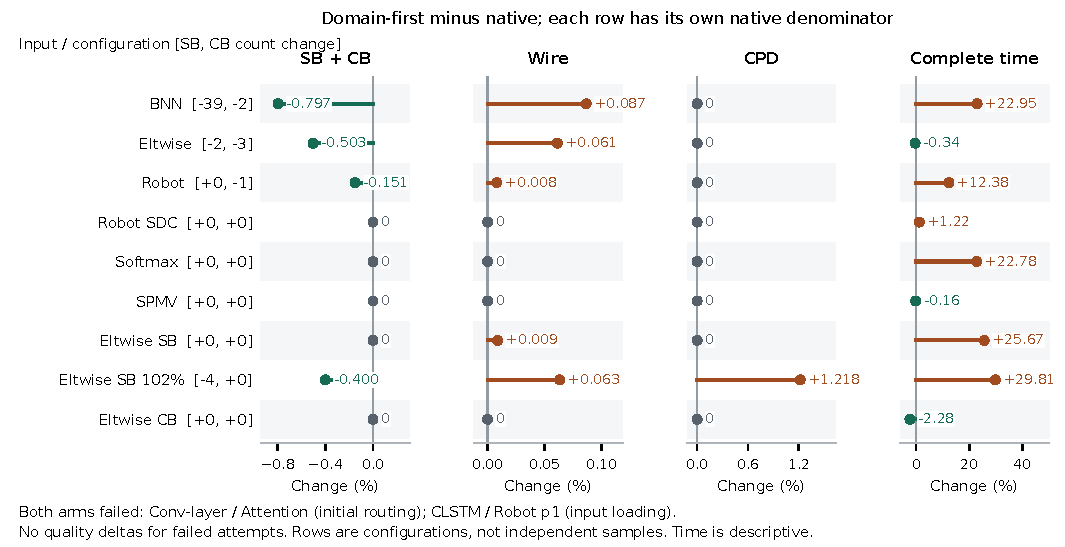
\includegraphics[width=.98\textwidth]{data/complete_paired_tradeoffs_10.pdf}
\caption{Complete domain-first/native tradeoffs from Table~\ref{tab:completecost}: $100(D-N)/N$ within each matched pair. Brackets report separate SB/CB count changes. Each panel has its own scale; lower is better for that metric. The BNN bar uses the original cold pair; balanced repeats are reported separately. Nine development configuration pairs are not nine independent inputs; the new no-op confirmation pair is reported in Table~\ref{tab:completecost}. Initial/input failures and grouped infrastructure failures retain costs without quality deltas. Single-run time differences are descriptive, not statistical speedups.}
\label{fig:joint}
\end{figure*}

The strong native A 0 BNN root is 13.607436067 ns,2059567 wire,94 SB,5062 CB. Three current-STA strict commits reduce CPD by 2.787376\% to 13.228145690 ns for 40 wire units, keeping vertical counts. The third step regresses a noncritical setup component; strict CPD and endpoint-vector rules therefore select different trajectories. Grouped repair can also improve a setup component when its first smaller subgroup is endpoint-flat and rejected. Complete group acceptance is essential to evaluating such combinations.

Figure~\ref{fig:joint} compares complete paired quality/cost, including no-gain cases. Older imported endpoints lack comparable complete times and receive no new cold costs. Local trajectories and full vectors remain supplementary; coincident points add no independent inputs.

Fixed terminal layers require 5103 counted nonglobal networks to cross. The audited graph has unit-capacity CB sources and uniquely paired unit-capacity SB halves. Distinct networks therefore require distinct counted resources: $S+C\ge 5103$. The 43-SB/5060-CB route attains that bound; under $C\le 5060$, $S\ge 43$ is attained. This is fixed-graph vertical occupancy optimality, with no claim of optimal placement, wire or timing.

A fixed timing envelope permits other useful points. On SB-only eltwise, setting the CPD limit once to 102\% of the root allows the domain branch to reach 995 SB,227583 wire and 6.114032 ns, versus native 999 SB,227439 wire and 6.040485 ns. It trades 144 wire,1.218\% CPD and 133.56 s for four fewer SB. The envelope is development-derived, not an external application requirement or unseen-test result. Both settings share the same initial trees and all 48 initial candidate records: changed timing budget, not different initial redundancy, permits this trade.

Terminal selection differs from transition acceptance: a Tf candidate saves 80 wire at fixed CPD/vertical counts but regresses four setup components. A three-net composition saves 24 wire with two setup improvements and no regression; FULL/STA and all 34 predicted delays agree. Imported validation costs 217.95 s. The separate complete terminal flow reaches 2059607/82/5062 at 13.228145690 ns in 7351.26 s, preserving the matched resource prefix/native work. Its qualified GNU-time is 7351/7247 s, +104 s; the old observer/PSS loss and overlap remain. This is a same-input tradeoff, not acceleration.

\section{Mechanism Ablations and Attribution}
\subsection{Domain restriction and failure release}
Matched domain controls fix source, request, scope and objective; each arm reselects after divergence. All nine BNN guided resource roles have passed audits and zero release events, as do eltwise/softmax. Their observed gains cannot be credited to executed release. Robot has five release events across three roles; its matched release-off ablations below provide the actual counterfactual. Events alone do not establish a whole-flow treatment effect.

In an R1 transaction, a guided net fails after five restorations. Capacity reachability is absent both immediately after pruning and at failure, whereas unrestricted search has a witness. This proves a fixed-scope/domain obstruction, not global unroutability.

Automatic release of only the failed network reproduces the selective-release route and full endpoint vector. It reaches 72 SB versus 74 for the matched unrestricted control, at 64 more wire and unchanged CPD/CB. Nine setup components improve with no regression; strict CPD rejects but endpoint-vector acceptance succeeds. Release preserves guidance for other networks, so its benefit must be separated from disabling all domains.

Robot's original 23-connection release-off transaction fails and restores its source exactly. A source-cut audit proves a conditional domain obstruction: outside owners occupy every same-layer exit, while the retained domain lacks a return crossing. Release enables search but does not remove those owners.

A new matched union holds the 25-connection/five-net scope fixed across unrestricted, domain/no-release and domain/release arms. No-release rolls back. Release yields 251160 wire/9 SB/653 CB at unchanged 13.354624073 ns, versus root 251161/10/653; 240 setup components improve, 32 regress, and hold violations do not increase. It passes the fixed resource-under-timing rule, but fails endpoint nonregression. Unrestricted yields 251140/9/654, improving 240 setup components without regression but exceeding the 653-CB cap. Thus retained domains alter the attainable tradeoff, and selective release restores feasibility within that domain; neither isolates a complete-controller gain. All are imported observations, with no actor commit. The shared command costs 194.52 s; cores are 3.00/1.62/4.45 s, not complete arm times.

\subsection{Blocking-owner coordination}
R 1's remaining excess crossing exposes a different limitation: all eight same-layer OPIN exits are owned by other nets. Fixed-scope trials preserve the extra crossing or fail with exact restoration; the 5104-resource state is a single-net local minimum. A current-margin selector adds one owner branch. Unrestricted and target-CB-domain transactions both reach 2070653 wire,32 SB,5071 CB, with the original full endpoint vector unchanged. Both transfer the blocking resource and attain the 5103 terminal bound. The observed benefit is expanded coordination scope; there is no additional domain advantage in this comparison.

In a same-source robot contrast, both searches are unrestricted with release disabled. Target-only yields 251173 wire,10 SB,653 CB; adding one owner yields 251185,10,654 at equal 13.354624073 ns. The added scope improves 31 setup components without regression but spends 12 wire/one CB. Endpoint acceptance permits it; fixed-resource acceptance rejects both, and neither is committed. The shared imported pair costs 155.10 s, not a cold flow. A capacity witness therefore motivates a proposal, not a resource-saving guarantee; smaller R1 alternatives remain in the supplement.

On robot-p1, four automatic unrestricted owner commits reenter the current state under the original root envelope: 231045/47/6677 becomes 231113/47/6673 at unchanged 11.633691344 ns. This trades 68 wire for four CB. One step regresses a setup component; resource acceptance does not require endpoint nonregression. Exact existing reload STA, endpoint identities and constraints match the source; a rounded display/manifest comparison caused a check failure. The trajectory remains incomplete development evidence, not domain attribution or fixed-version confirmation.

\subsection{Grouping and complete combinations}
Transaction count is not a cost proxy: K 8/budget64 execute the same query multiset in 18/32 transactions at 7099.32/10568.53 s; a proposed-query heuristic costs 10308.49 s at equal CPD/SB/CB. These imported controls show no benefit.

Tied-path feedback supplies a complementary positive combination example. Jointly covering two tied-path targets with three donors improves ten setup components with no regression, gaining 7.638334 ps at 45 SB/5060 CB. A larger successor improves CPD further but regresses a noncritical setup component. The policy distinction is deliberate, and neither result establishes that every intermediate or module should improve CPD. Historical local trajectories and recovery costs are retained in the supplement.
\section{Overhead and Applicability}
\subsection{Engineering cost and symmetric controls}
Behavior-preserving indexing/streaming observations, including the qualified 7247-s GNU-time run, remain supplementary. With identical engineering, serial N/D/D/N gives mean complete times 7308.61/9129.25 s: ratio 1.24911, or 24.91\% domain overhead. Paired ratios are 1.24796/1.25026. Same-role trajectories, full requests, native work and six actual graph payloads match; paired fresh roots/full endpoint vectors match, with compatible final endpoint comparisons. Missing memory observations are 22/28/27/29 in registered order. Four whole repeats add no independent input. Two observations per arm on a shared host with uncontrolled OS caches support descriptive costs only. The original 22.95\% overhead is retained as a separate historical observation; no component times are summed or observer CPU subtracted.

In the original BNN pair, resource transactions account for 1692.84 s of the observed 1821.07-s total difference (92.96\%). Native/domain execute 70/1361 connection queries, counting repeated queries separately. Nested native-core times are 38.23/1207.26 s and cannot be added to complete costs. This decomposition identifies the dominant work, not a new speedup.

Lazy scheduling skips optional native diagnostics only after complete domain acceptance. Eltwise preserves states/candidates with 64$\to$32 queries, 101$\to$51 attempts and 203.48 versus 289.21 s; softmax takes 271.70 versus 336.68 s. SPMV has no skipped work and takes 93.15 versus 91.55 s. Source snapshots further give 198.88/256.54 s on eltwise/softmax. Fused FULL/STA alone instead costs 313.74 versus 289.21 s on eltwise. Complete controls, not process counts, establish engineering benefit.



Complete times bind commands/outputs; shared-host activity and caches remain uncontrolled. Interleaving retains failures; recovery and validation costs stay separate.

\subsection{Evidence coverage and confirmation boundary}
The historical 671-record archive has 34 quality-complete configurations, not independent samples: 33 observer measurements and one qualified GNU-time. Fourteen later terminal attempts, four balanced timing repeats, nine infrastructure failures and five scoped components lie outside those counts. Failed roles have no legal quality; sampled PSS may miss transient peaks. Full trajectories, vectors and per-arm failure costs remain supplementary.

Corrected CLSTM N/D, robot-p1 N and reduction N/D reach legal initial routes before supervision interruption. Four CP1r1 attempts fail guard launch before VPR. Original failures/costs remain. CP1r2 fixes runtime supervision and permissions; actual guard tests/public reconstruction pass without algorithm changes.

Applicability is limited to two-layer edge-encoded Hybrid-O/SB-only/CB-only. Flat routing, CHANZ, general multilayer and broad constrained application suites remain unconfirmed. The altered robot placement adds one no-gain input. CB-only attains its 982-source terminal bound, without wire/CPD optimality.

CP1/CP1r2 bind source, dependencies, binaries, mechanism order, root envelopes and terminal policy; native has matching opportunities. Prospective input/configuration seals precede outcomes; revisions require new releases. The robot union separates domain/release at one fixed scope; cross-input confirmation remains necessary. Input identity includes netlist, architecture, placement, constraints and trees; identical-tree seeds add no starts. BNN defaults and robot SDC~\cite{vprsdc} establish no external application requirement.

The evidence supports specific complete-flow tradeoffs and local mechanisms, not broad controller superiority, timing-closure guarantees or statistical acceleration.
\begin{thebibliography}{9}
\bibitem{vtr9paper} M. A. Elgammal et al., ``VTR 9: Open-source CAD for fabric and beyond FPGA architecture exploration,'' \emph{ACM Trans. Reconfigurable Technol. Syst.}, 2025, doi:10.1145/3734798.
\bibitem{lazagna} I. Youssef, H. Yang, and C. Hao, ``LaZagna: An open-source framework for flexible 3D FPGA architectural exploration,'' in \emph{Proc. ICCAD}, 2025, pp.1--9, doi:10.1109/ICCAD66269.2025.11240893.
\bibitem{flatland} C. Hao, A. B. Kahng, B. Pramanik, and I. Youssef, ``Escaping Flatland: A placement flow for enabling 3D FPGAs,'' in \emph{Proc. ACM/IEEE DAC}, 2026, doi:10.1145/3770743.3804424.
\bibitem{pathfinder} L. McMurchie and C. Ebeling, ``PathFinder: A negotiation-based performance-driven router for FPGAs,'' in \emph{Proc. FPGA}, 1995, pp.111--117.
\bibitem{liurepair} Y. Liu, H. Yang, W. Yu, X. Cui, and J. Huang, ``An FPGA timing routing algorithm based on PathFinder and rip-up and retry approach,'' \emph{J. Computer-Aided Design \& Computer Graphics}, vol.26, no.1, pp.138--145, 2014.
\bibitem{air} K. E. Murray, S. Zhong, and V. Betz, ``AIR: A fast but lazy timing-driven FPGA router,'' in \emph{Proc. ASP-DAC}, 2020, pp.338--344.
\bibitem{croute} D. Vercruyce, E. Vansteenkiste, and D. Stroobandt, ``CRoute: A fast high-quality timing-driven connection-based FPGA router,'' in \emph{Proc. FCCM}, 2019, pp.53--60, doi:10.1109/FCCM.2019.00017.
\bibitem{multidie} A. Poolad, S. Gholami Shahrouz, A. Boutros, and V. Betz, ``Modeling, optimizing and exploring multi-die FPGA routing architectures,'' arXiv:2606.06421v3, 2026.
\bibitem{vprsdc} Verilog-to-Routing, ``Timing constraints,'' \url{https://docs.verilogtorouting.org/en/latest/vpr/timing_constraints/}, accessed Nov.15,2026.
\end{thebibliography}
\end{document}
